\documentclass{article}
\usepackage{graphicx}
\usepackage{amssymb}
\usepackage{amsmath}
\usepackage{parskip}
\usepackage{tabularray}
\usepackage[a4paper,margin=1.25cm]{geometry}

\newcounter{problem}
\newcounter{extraproblem}
\newcommand{\question}[1]{\refstepcounter{problem}\par\smallskip\textbf{T\theproblem.}\quad #1\par\smallskip}
\newcommand{\extraquestion}[1]{\refstepcounter{extraproblem}\par\smallskip\textbf{OT\theextraproblem.}\quad #1\par\smallskip}

\begin{document}
\title{Homework 1 Clustering and Regression}
\author{Nipat Chenthanakij 6430215121}
\date{}
\maketitle
\subsection*{Metrics}
\begin{center}
    \begin{tblr}{hlines,vlines}
        Model A    & Predicted dog & Predictted cat \\
        Actual dog & 30            & 20             \\
        Actual cat & 10            & 40
    \end{tblr}
\end{center}

\question{What is the accuracy of Model A?}
Accuracy = \(\dfrac{TP+FP}{TP+TN+FP+FN} = \dfrac{30+40}{30+20+10+40}=0.7\).

\question{Consider cats as 'class 1' (positive) and dogs as 'class 0' (negative). Calculate the precision, recall, and F1.}
Precision = \(\dfrac{TP}{TP+FP} = \dfrac{40}{20+40} = \dfrac23\)

Recall = \(\dfrac{TP}{TP+FN} = \dfrac{40}{10+40} = \dfrac45\)

F1 = \(2 \times \dfrac{\text{precision} \times \text{recall}}{\text{precision} + \text{recall}} = 2 \times \dfrac{\dfrac23 \times \dfrac45}{\dfrac23 + \dfrac45} = \dfrac{8}{11}\)

\question{Consider class cat as 'class 0' and class dog as 'class 1', calculate the precision, recall, and F1.}
Precision = \(\dfrac{TP}{TP+FP} = \dfrac{30}{30+10} = \dfrac34\)

Recall = \(\dfrac{TP}{TP+FN} = \dfrac{30}{30+20} = \dfrac35\)

F1 = \(2 \times \dfrac{\text{precision} \times \text{recall}}{\text{precision} + \text{recall}} = 2 \times \dfrac{\dfrac34 \times \dfrac35}{\dfrac34 + \dfrac35} = \dfrac23\)

\question{Consider a lopsided population where there are 80\% cats. What is the accuracy of model A? Using dog as the positive class, what is the precision, recall, and F1?
    Explain how and why these numbers change (or does not change) from the previous questions.}
\extraquestion{Consider the equations for accuracy and F1
    \begin{align*}
        \text{Accuracy} & = \dfrac{TP+FP}{TP+TN+FP+FN} \\
        F1              & = \dfrac{2TP}{2TP+FP+FN}
    \end{align*}
    When will accuray be equal, greater, or less than F1?
}
\subsection*{Hello Clustering}
\question{If the starting points are (3,3), (2,2), and (-3,-3). Describe each
    assign and update step. What are the points assigned? What are the updated
    centroids? You may do this calculation by hand or write a program to do it.}
\begin{center}
    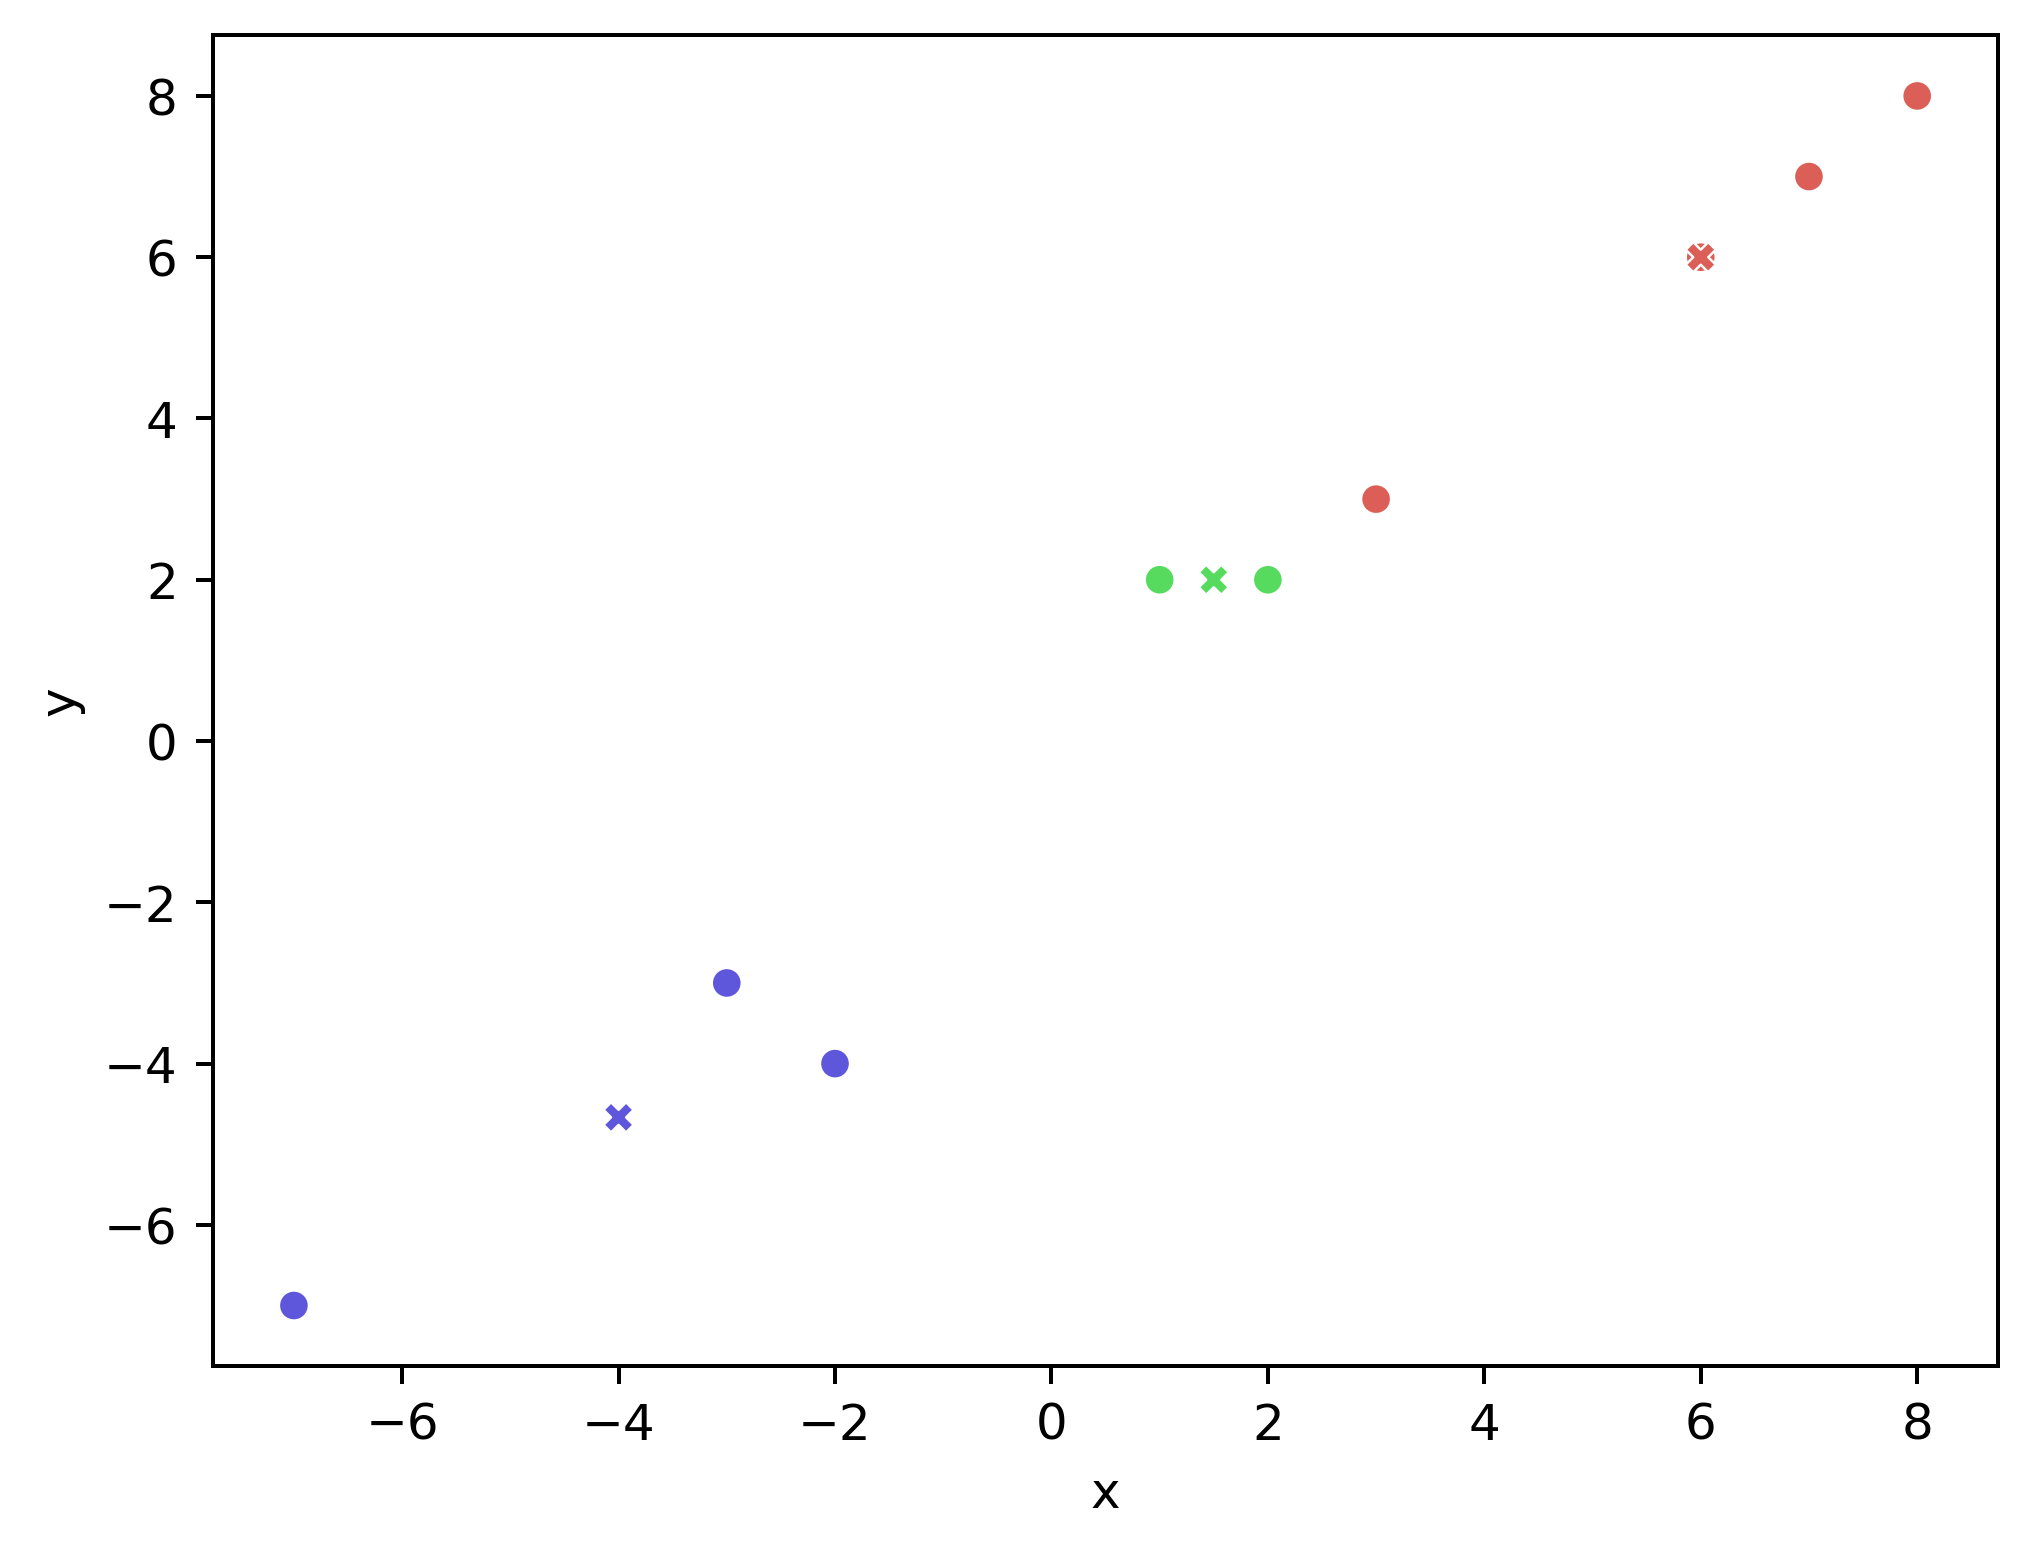
\includegraphics[width=0.5\textwidth]{img/kmean00.png}
    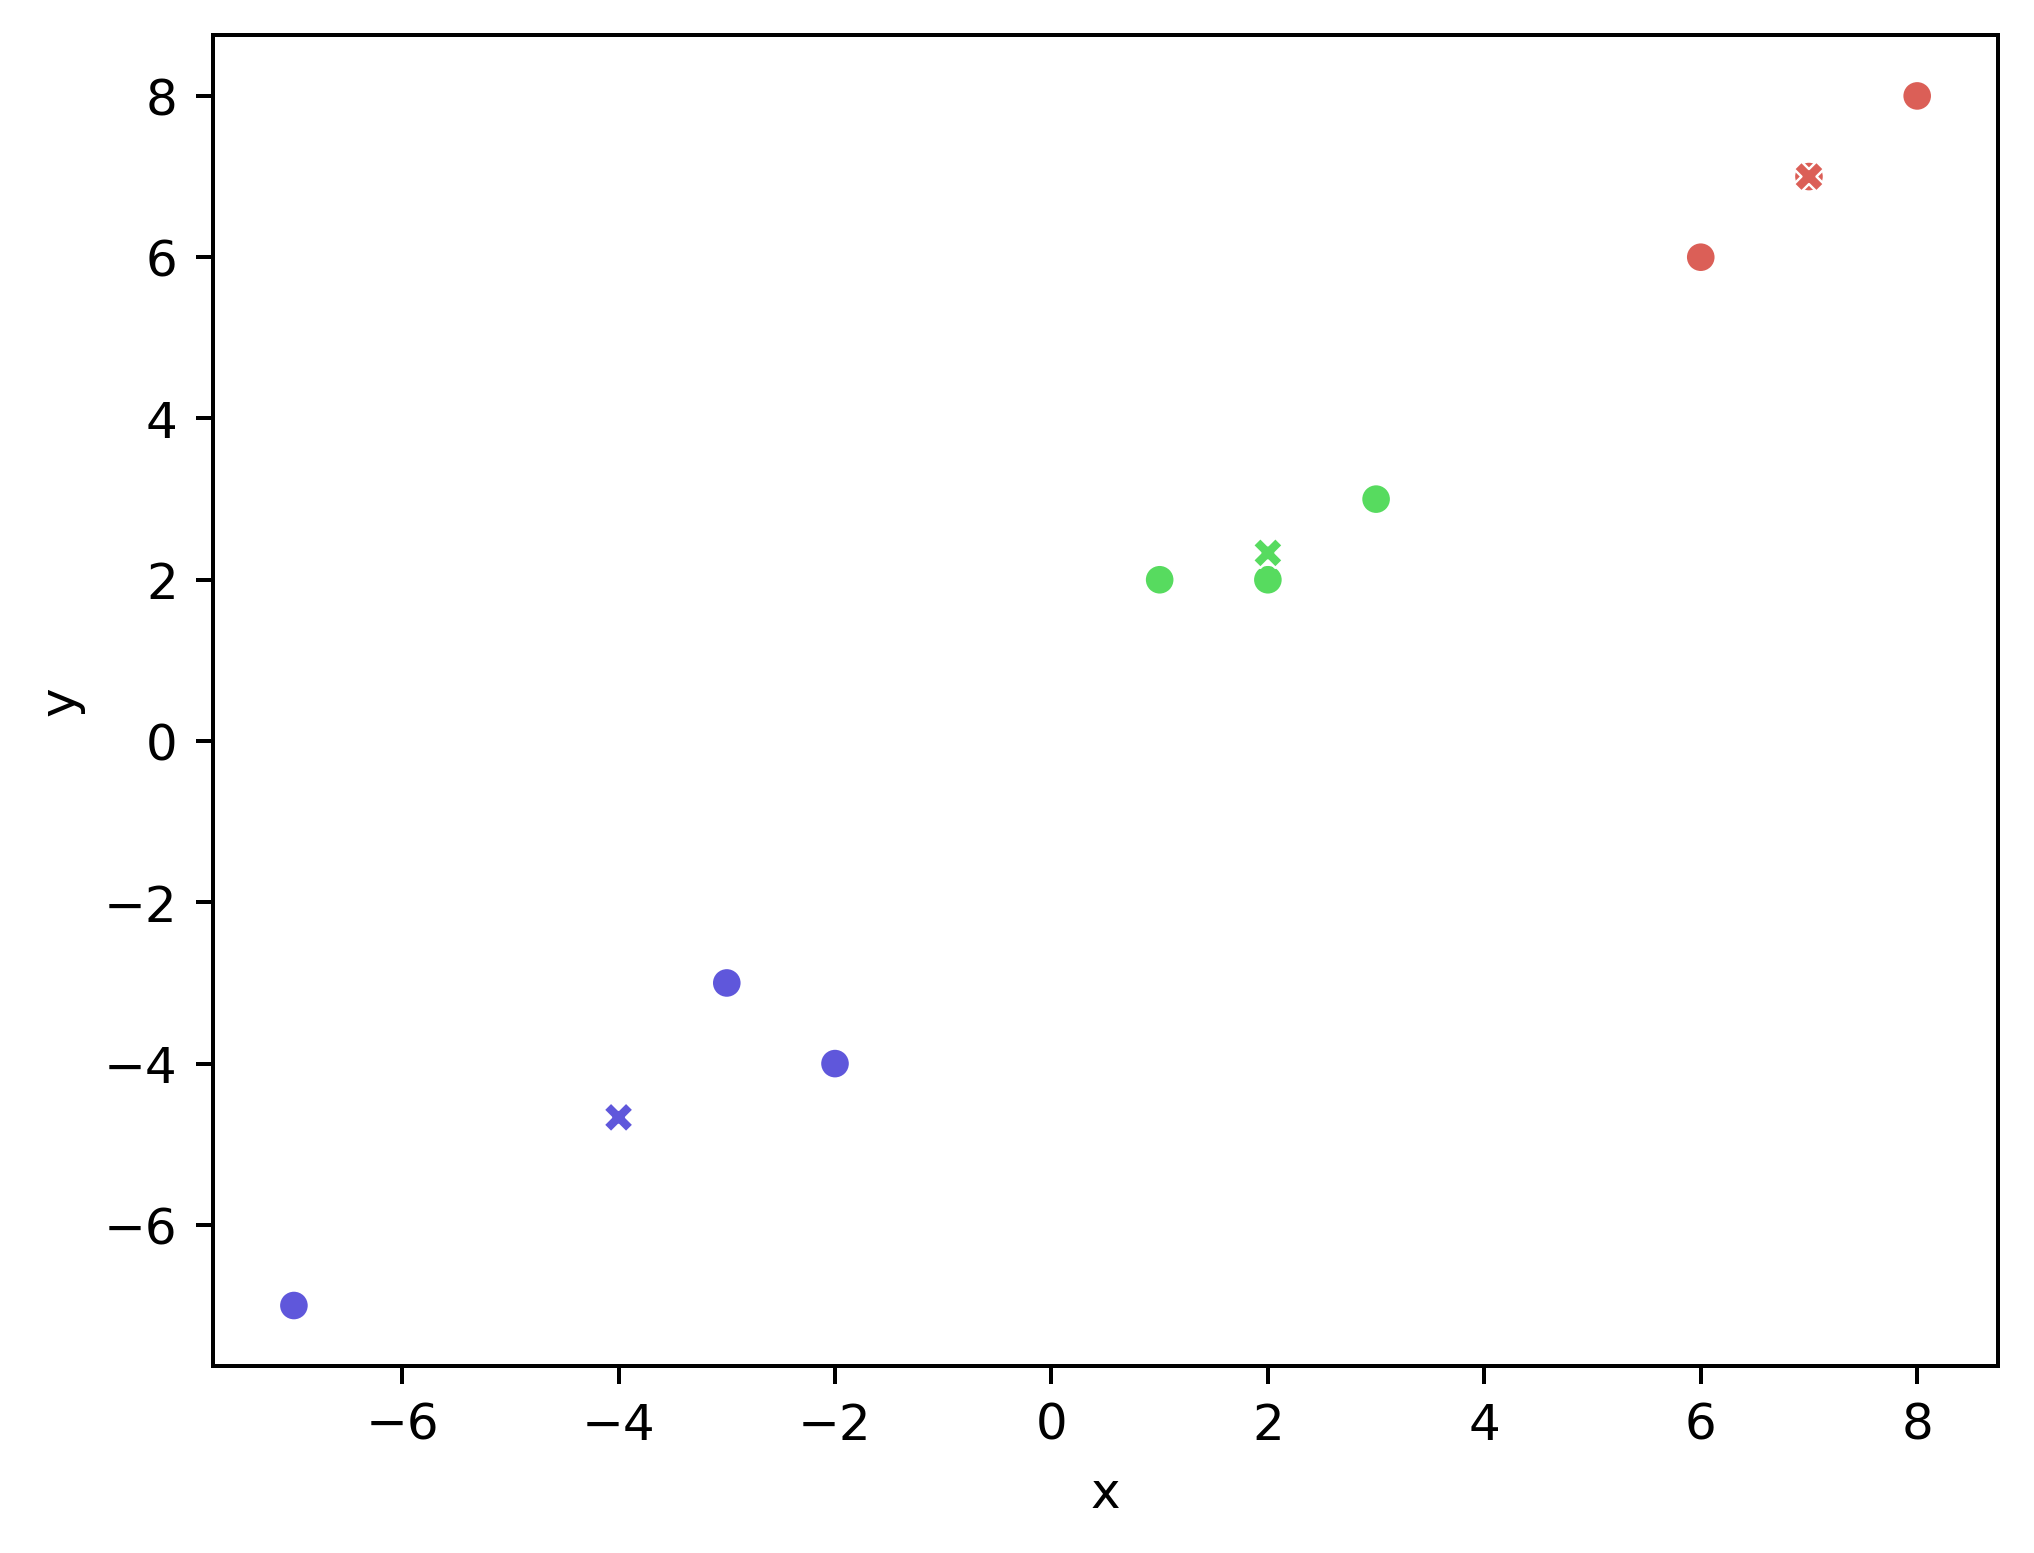
\includegraphics[width=0.5\textwidth]{img/kmean01.png}
\end{center}
\question{If the starting points are (-3,-3), (2,2), and (-7,-7), what happens?}
\begin{center}
    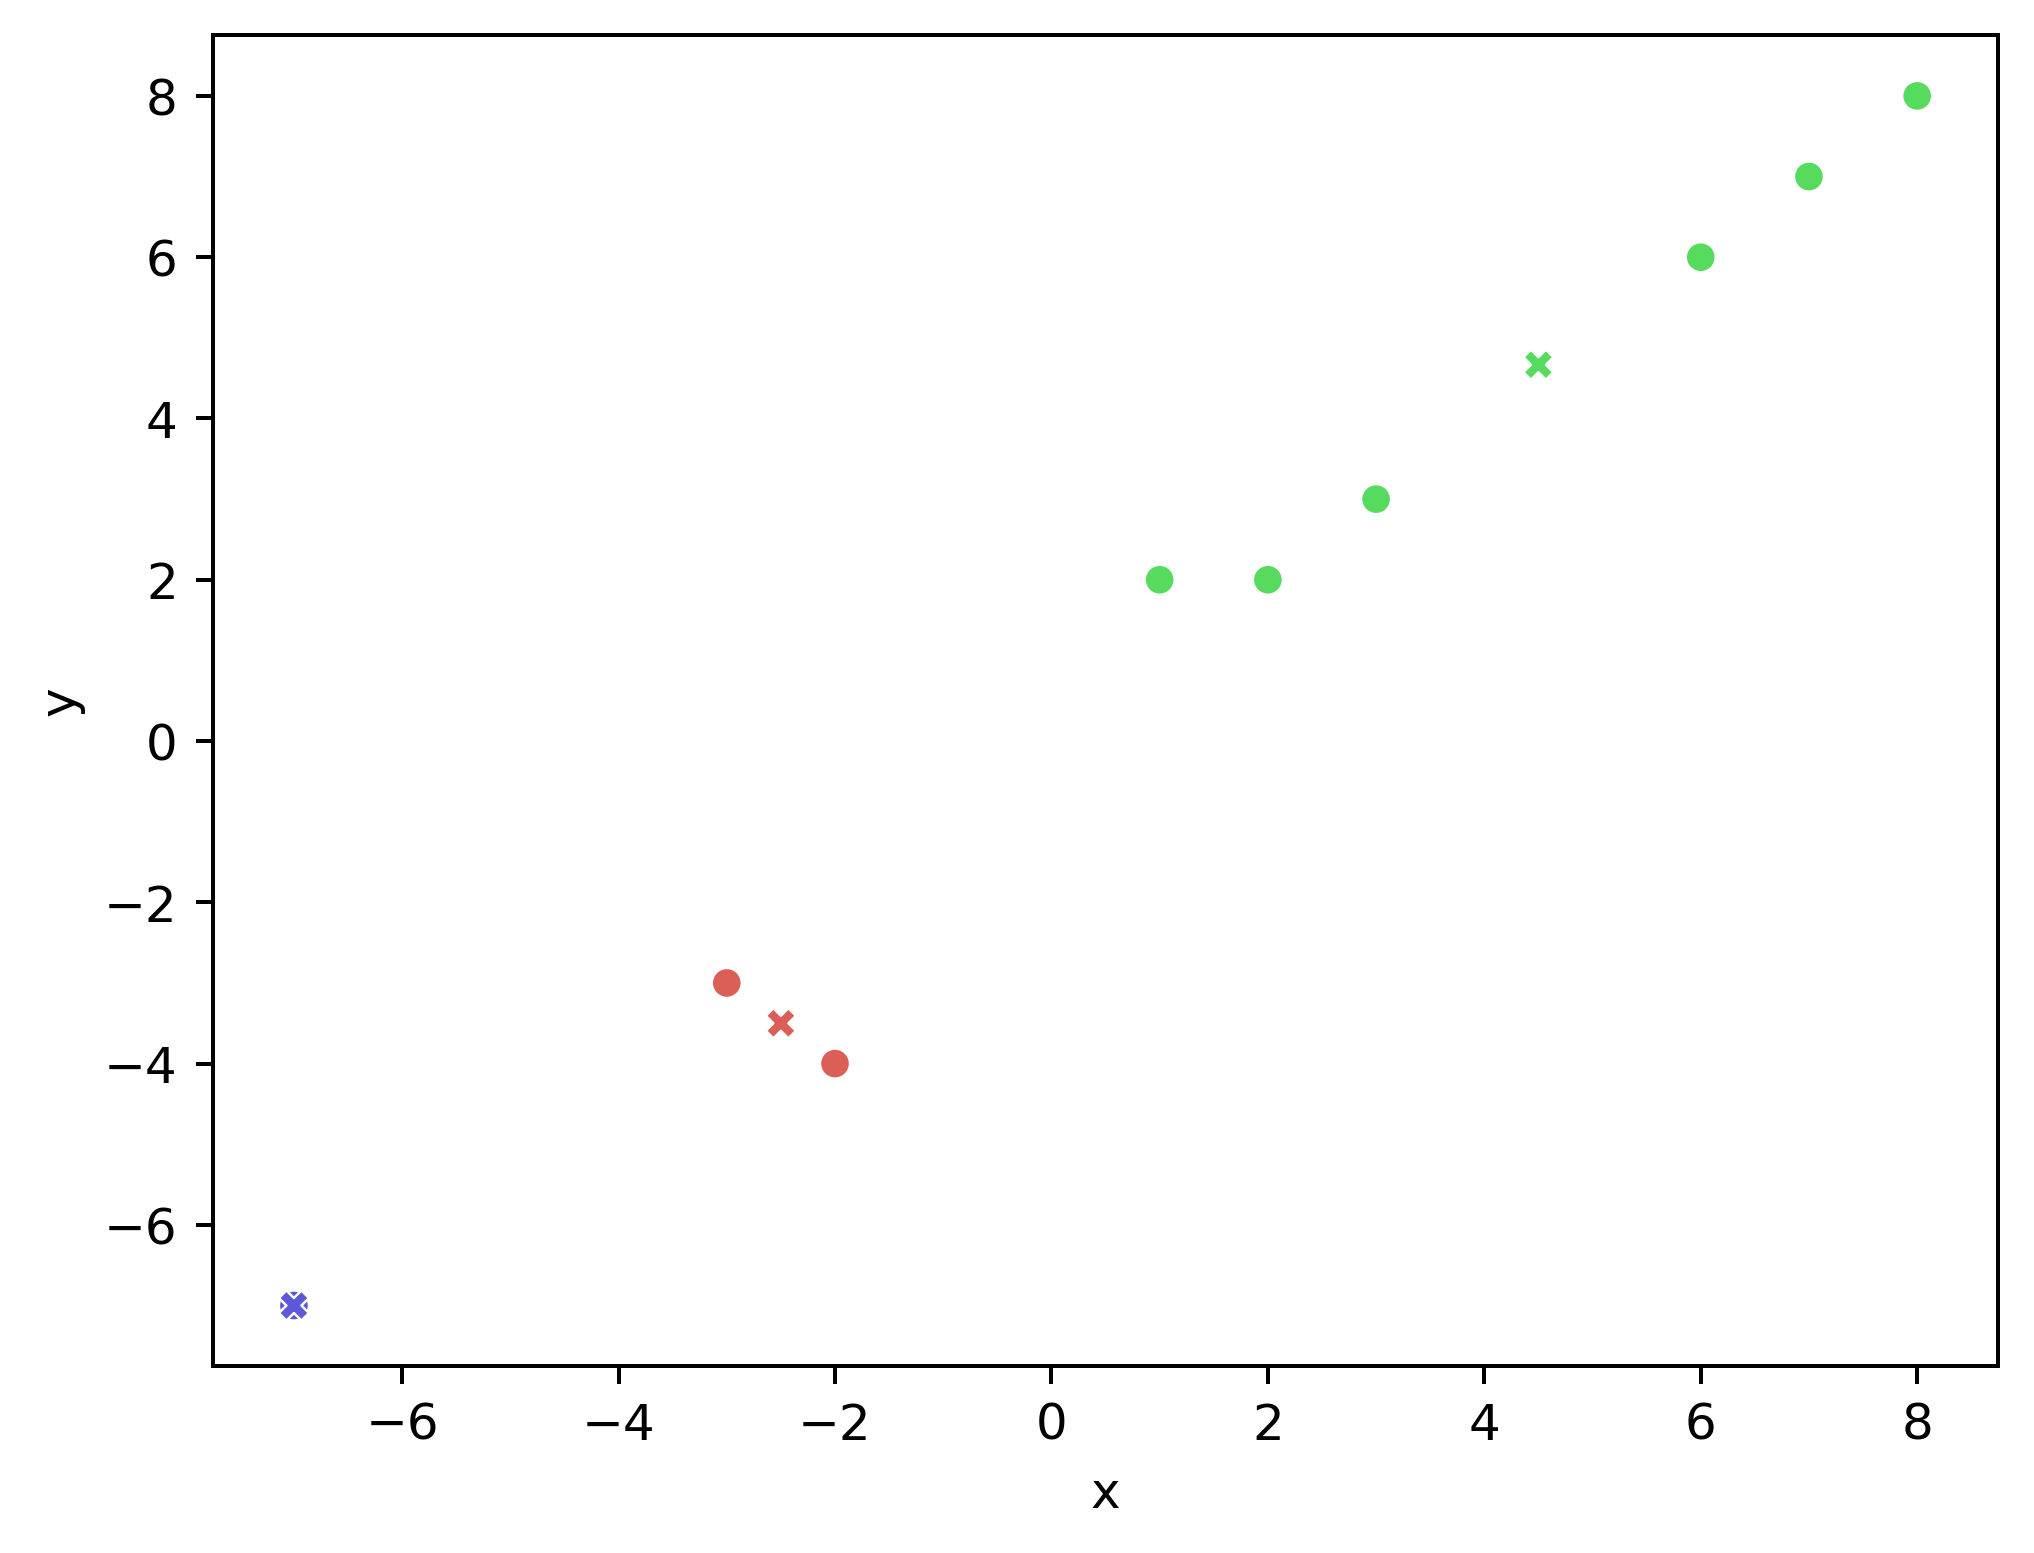
\includegraphics[width=0.5\textwidth]{img/kmean10.png}
\end{center}
\question{Between the two starting set of points in the previous two questions,
    which one do you think is better? How would you measure the 'goodness' quality
    of a set of starting points?}
\extraquestion{What would be the best K for this question? Describe your reasoning.}
\subsection*{My heart will go on}
\question{What is the median age of the training set?}
\question{Some fields like 'Embarked' are categorical. They need to be converted
    to numbers first. We will represent S with 0, C with 1, and Q with 2. What is
    the mode of Embarked? Do the same for Sex.}
\question{Write a logistic regression classifier using gradient descent as learned
    in class. Use PClass, Sex, Age, and Embarked as input features.}
\question{Submit a screenshot of your submission (with the scores). Upload
    your code to courseville.}
\question{Try adding some higher order features to your training (\(x_1^2\), \(x_1 x_2\), ...).
    Does this model has better accuracy on the training set? How does it
    perform on the test set?}
\question{What happens if you reduce the amount of features to just Sex and Age?}
\extraquestion{We want to show that matrix inversion yields the same answer
    as the gradient descent method. However, there is no closed form solution for
    logistic regression. Thus, we will use normal linear regression instead. Redo
    the Titanic task as a regression problem by using linear regression. Use the
    gradient descent method.}
\extraquestion{Now try using matrix inversion instead. However Are the weights
    learned from the two methods similar? Report the Mean Squared Errors (MSE)
    of the difference between the two weights.}
\end{document}